The central research question of this project was whether currently available, student-accessible quantum computing platforms are sufficiently mature to meaningfully implement Grover’s algorithm for nontrivial problems such as games and puzzle-like search tasks. Across all experiments, a clear distinction emerges between theoretical performance, simulation results, and execution on real quantum hardware.

\vspace{1em}
\noindent
In ideal, noise-free simulations, Grover’s algorithm consistently behaves as expected: valid solutions are amplified according to theoretical predictions, and the correct configurations dominate the measurement outcomes near the optimal number of iterations. These results confirm that the problem encodings, oracle constructions, and diffusion operators are logically correct and that Grover’s algorithm can, in principle, be applied to structured problems beyond textbook examples.

\vspace{1em}
\noindent
When moving from simulation to realistic noise models and real quantum hardware, performance degrades significantly. While small instances occasionally retain partial amplification, increasing circuit depth and the number of multi-qubit gates quickly leads to decoherence and loss of signal. In practice, circuit depth, rather than raw qubit count, emerges as the dominant limiting factor. Compilation overhead, connectivity constraints, and accumulated gate errors often eliminate the theoretical advantage predicted by Grover’s algorithm.

\vspace{1em}
\noindent
These results indicate that, although Grover’s algorithm is theoretically applicable to game-like problems, its practical usefulness on current student-accessible quantum hardware is limited to very small problem instances. Larger instances remain feasible only in simulation, where hardware noise and coherence constraints are absent.

\vspace{1em}
\noindent
The following sections report the results separately for each studied problem.

\paragraph{Sudoku:}
The solver was first executed on a $2\times 2$ Sudoku instance using IBM quantum hardware. Due to the small problem size, the resulting circuit depth was well within the coherence time of the processor. As shown in Figure~\ref{fig:2x2_hardware}, the hardware successfully identified the correct solutions. While it is clearly visible that noise is present, and it is manifesting as non-zero probabilities for invalid states, the bitstrings of the correct solutions stand out with a statistically significant probability peak.

\begin{figure}[H]
    \centering
    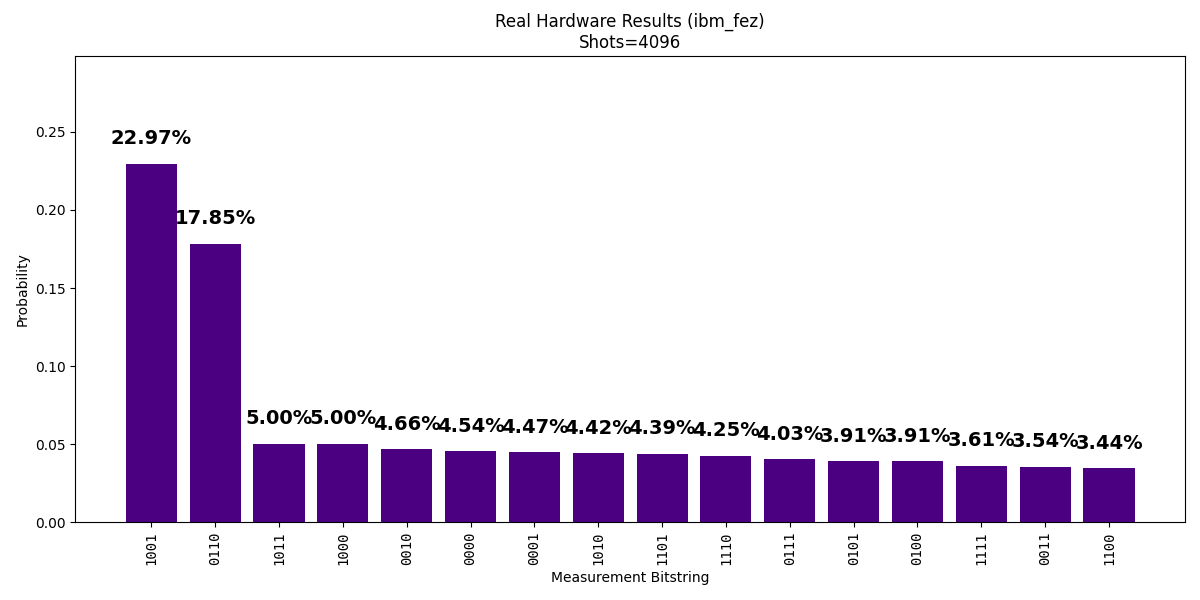
\includegraphics[width=1\linewidth]{ibm_hardware_result_2x2.png}
    \caption{Hardware results for the $2\times 2$ Sudoku instance. Unlike the larger case, the circuit depth here is shallow enough that the signal survives decoherence. Both highest bars represent the valid solutions, and are clearly distinguishable from the noise.}
    \label{fig:2x2_hardware}
\end{figure}

% \begin{figure}
%     \centering
%     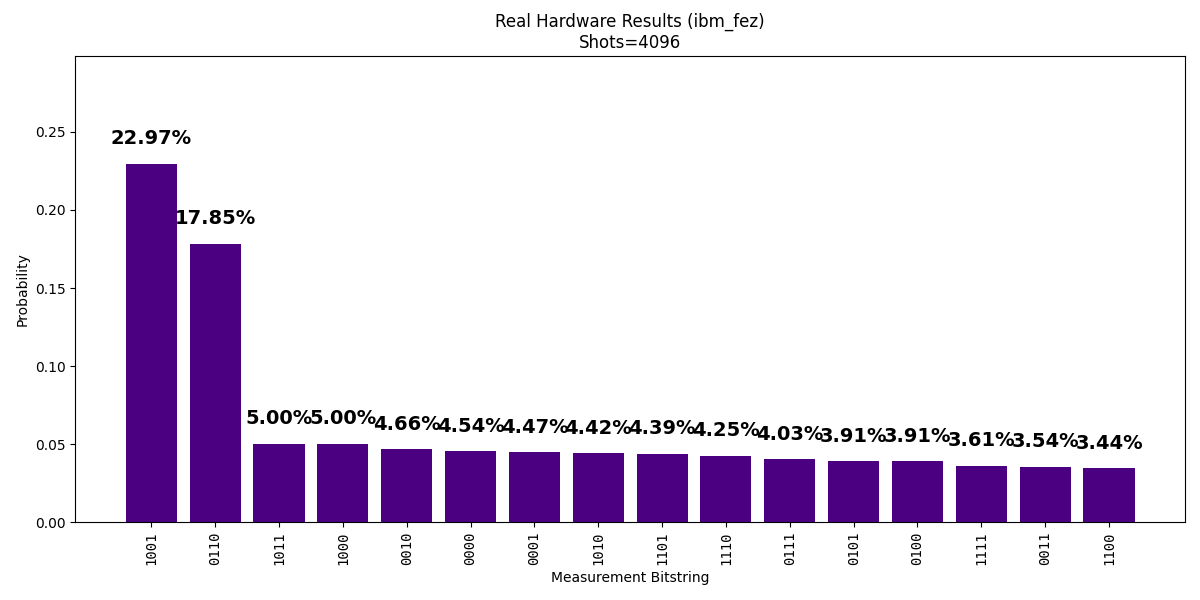
\includegraphics[width=1\linewidth]{ibm_hardware_result_2x2.png}
%     \caption{Enter Caption}
%     \label{fig:placeholder}
% \end{figure}

% \vspace{1em}
% \noindent
% The hardware results show the expected Grover amplification pattern: the correct solutions appear more frequently near the predicted number of iterations, but with a lower success probability than the simulator due to noise and decoherence of the quantum hardware on which the code is run. Because Grover is probabilistic, probabilities are reported by dividing the measured outcomes by the shot count. The following histogram summarizes the hardware measurements for both the $2\times 2$ and the partially filled $4\times 4$ runs.

% \vspace{1em}
\noindent
Following the successful proof of concept, the Grover search for the partially filled $4\times 4$ Sudoku (6 unknowns) was executed on both a noiseless simulator and the \texttt{ibm\_torino} quantum processor. The logical circuit required approximately 28,000 quantum gates and was set to run for 50 iterations, the theoretically optimal number calculated for this problem size.

\begin{figure}[H]
    \centering
    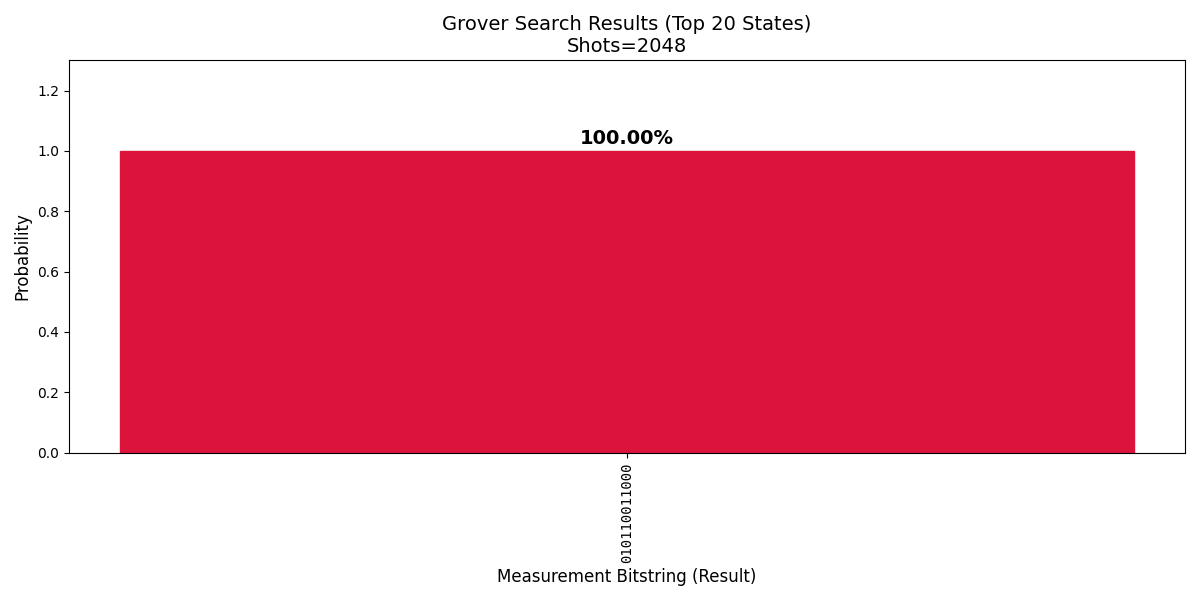
\includegraphics[width=1\linewidth]{Simulator_2.png}
    \caption{Ideal simulation results (50 Iterations). In the absence of noise, Grover's algorithm converges to the correct state with unity probability, serving as the theoretical baseline for hardware comparisons.}
    \label{fig:sim_50}
\end{figure}

\vspace{1em}
\noindent
The algorithm was run on the Qiskit Aer Statevector simulator. Figure~\ref{fig:sim_50} demonstrates the algorithm's logical correctness: the probability of measuring the correct solution state (\texttt{010110011000}) reached 100\%, confirming that the Oracle and Diffuser were constructed correctly and capable of amplifying the solution in a noise-free environment. Moreover, using a less than theoretically optimal number of iterations shows the expected Grover amplification pattern \cite{BoscoLecture5} (e.g., 97.61\% at 45 iterations, see Figure~\ref{fig:sim_45}, 51.61\% at 25 iterations, see Figure~\ref{fig:sim_25}, and $\sim0.0035\%$ at only one iteration, see Figure~\ref{fig:sim_1}), thus validating the theoretical model.

\begin{figure}[H]
    \centering
    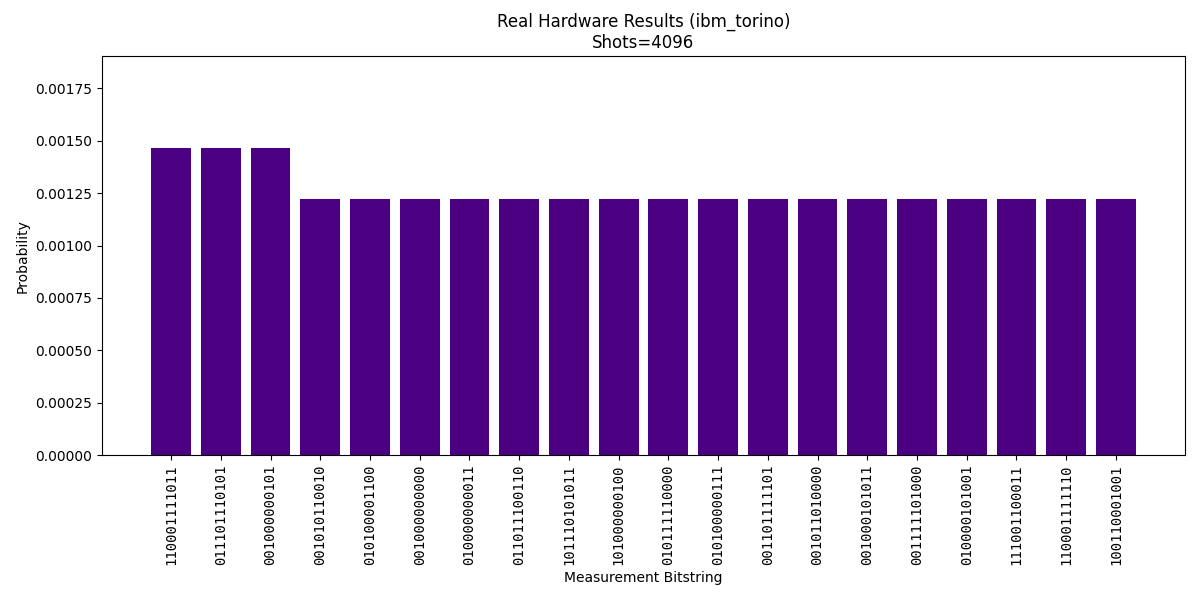
\includegraphics[width=1\linewidth]{ibm_hardware_result.png}
    \caption{Experimental results on \texttt{ibm\_torino} (4096 shots). The distribution is flat, indicating that the quantum state decohered into random noise before the computation could complete.}
    \label{fig:ibm_4x4}
\end{figure}

\noindent
When the circuit was executed on the \texttt{ibm\_torino} backend (133 qubits), the results were drastically different. As shown in Figure~\ref{fig:ibm_4x4}, the probability distribution is indistinguishable from uniform random noise ($\sim$0.015\%). The amplification observed in the simulator was completely lost.

\vspace{1em}
\noindent
To understand the discrepancies between the simulation and the hardware execution, the circuit compilation and the probability of the algorithm to find the correct answer were analyzed in both theoretical and real scenarios.

\begin{figure}[H]
    \centering
    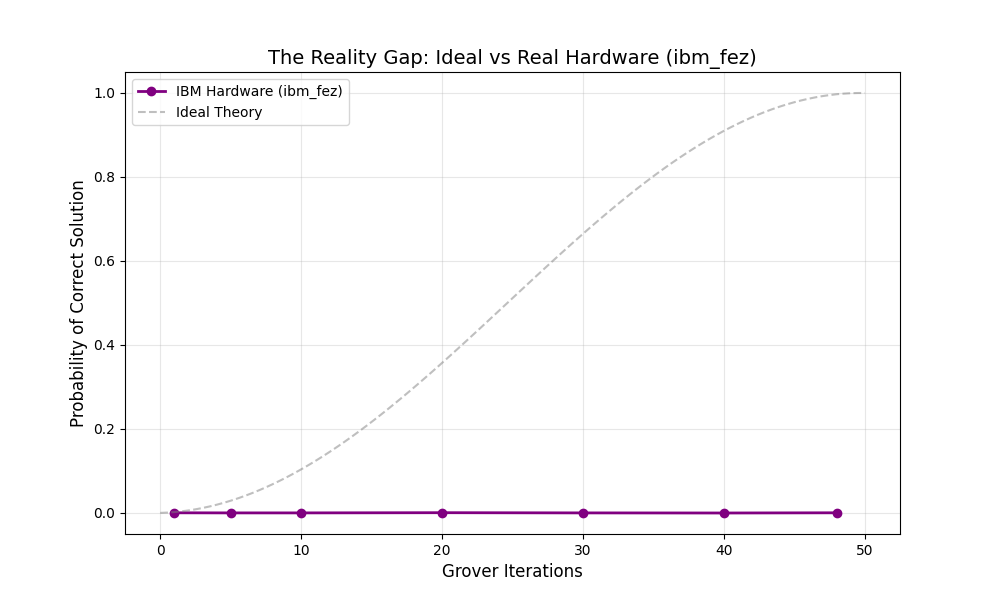
\includegraphics[width=1\linewidth]{ibm_death_curve.png}
    \caption{Coherence limit analysis. The ideal probability (grey) rises to 100\%, while the real hardware probability (purple) never deviates from zero, showing that noise dominates the signal instantly.}
    \label{fig:death_curve}
\end{figure}

\noindent
A depth-sweep experiment was performed, running the algorithm for $k \in \{1, 5, \ldots, 50\}$ iterations on hardware. Figure~\ref{fig:death_curve} illustrates the gap between the simulation and the real capabilities of a current quantum computer. While theory predicts a smooth sinusoidal rise in probability (grey line), the hardware success rate (purple line) remains flat at zero even for shallow depths. This indicates that the circuit depth exceeded the qubit coherence time ($T_1/T_2$) almost immediately.

\vspace{1em}
\noindent
The primary cause of this failure was identified in the transpilation phase of the process. The logical circuit contained approximately 28{,}100 gates, and to map this to the physical hardware, the insertion of SWAP gates was required to satisfy connectivity constraints. This caused a massive increase in the gate count to 785{,}780 and the circuit depth to 290{,}053. Given that current superconducting qubits can typically sustain only a few thousand gates before decoherence, a depth of 290{,}000 makes successful computation physically impossible for the currently available hardware.

\paragraph{Lights Out:}
The Lights Out Grover implementation was executed on three execution targets and the outcome distributions were compared: (1) a noiseless statevector simulator, (2) the Qiskit fake backend \texttt{FakeMarrakesh} (which includes simulated noise), and (3) real IBM hardware (\texttt{ibm\_marrakesh}).

\vspace{1em}
\noindent Key numerical results for the $2\times 2$ instance (initial game state \texttt{1001}, correct solution \texttt{1001}):
\begin{itemize}
	\item Perfect (statevector) simulator, 100k shots: measured solution frequency $\approx 96.13\%$; second-most frequent outcome was \texttt{1000} at $\approx 0.28\%$.
	\item \texttt{FakeMarrakesh} noise simulation, 10k shots: measured solution frequency $\approx 37.61\%$; second-most frequent outcome was \texttt{1011} at $\approx 6.03\%$.
	\item Real hardware (\texttt{ibm\_marrakesh}), 100k shots: measured solution frequency $\approx 16.42\%$; second-most frequent outcome was \texttt{0001} at $\approx 6.90\%$ (significant degradation compared to the simulator).
\end{itemize}

\noindent
Before transpilation for IBM hardware, the circuit had 156 gates and the depth was 63. After transpilation for the target hardware, the circuit grew to 3287 gates with a depth of 971. The large increase in two-qubit operations (e.g., SWAP gates introduced due to connectivity constraints) dramatically increased circuit depth and size. This increase is the main contributor to the loss of signal on hardware.

\noindent
Additionally, since the transpilation is non-deterministic, the amount of gates and the circuit's depth are random. Therefore, a good transpilation seed was found to minimize the depth of the circuit.

\vspace{1em}
\noindent
The simulator run confirms the correctness of the oracle and diffuser (see Figure~\ref{fig:lights_out_histograms}). The noisy simulator shows that, under a realistic noise model, some amplification survives, whereas the hardware execution suffers from decoherence and compilation overhead.

\begin{figure}[H]
	\centering
	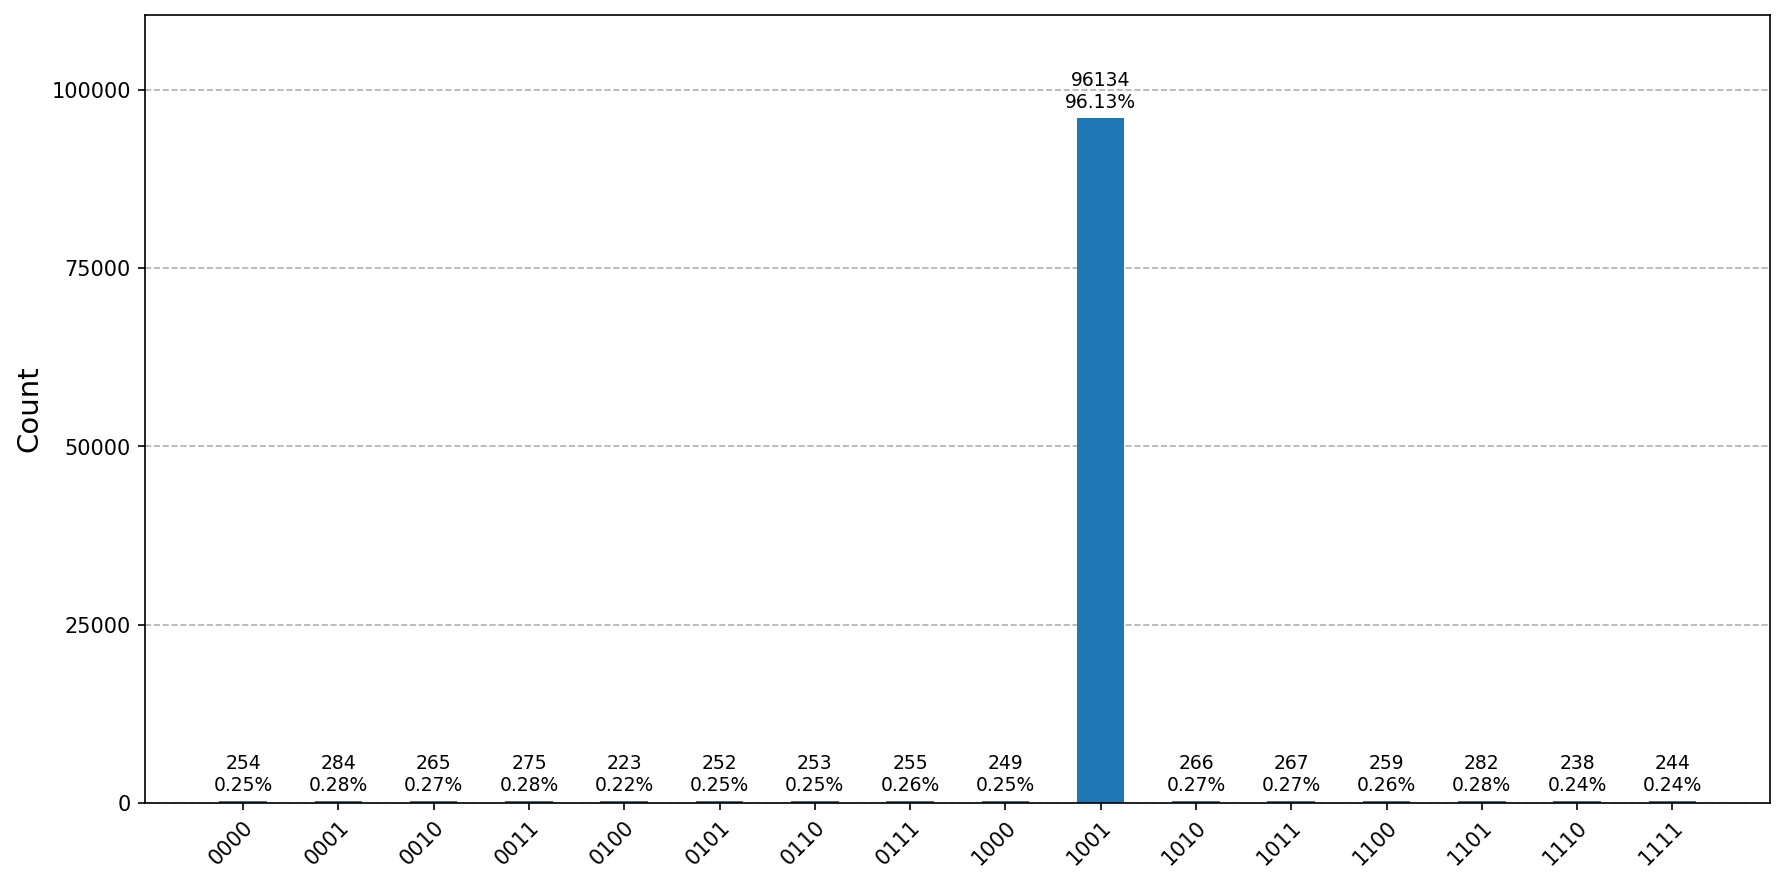
\includegraphics[width=\columnwidth]{figures/lights_out/perfect_simulator_100k.png}\\
	{\small (a) Perfect statevector simulator (100k shots)}\\[0.8em]
	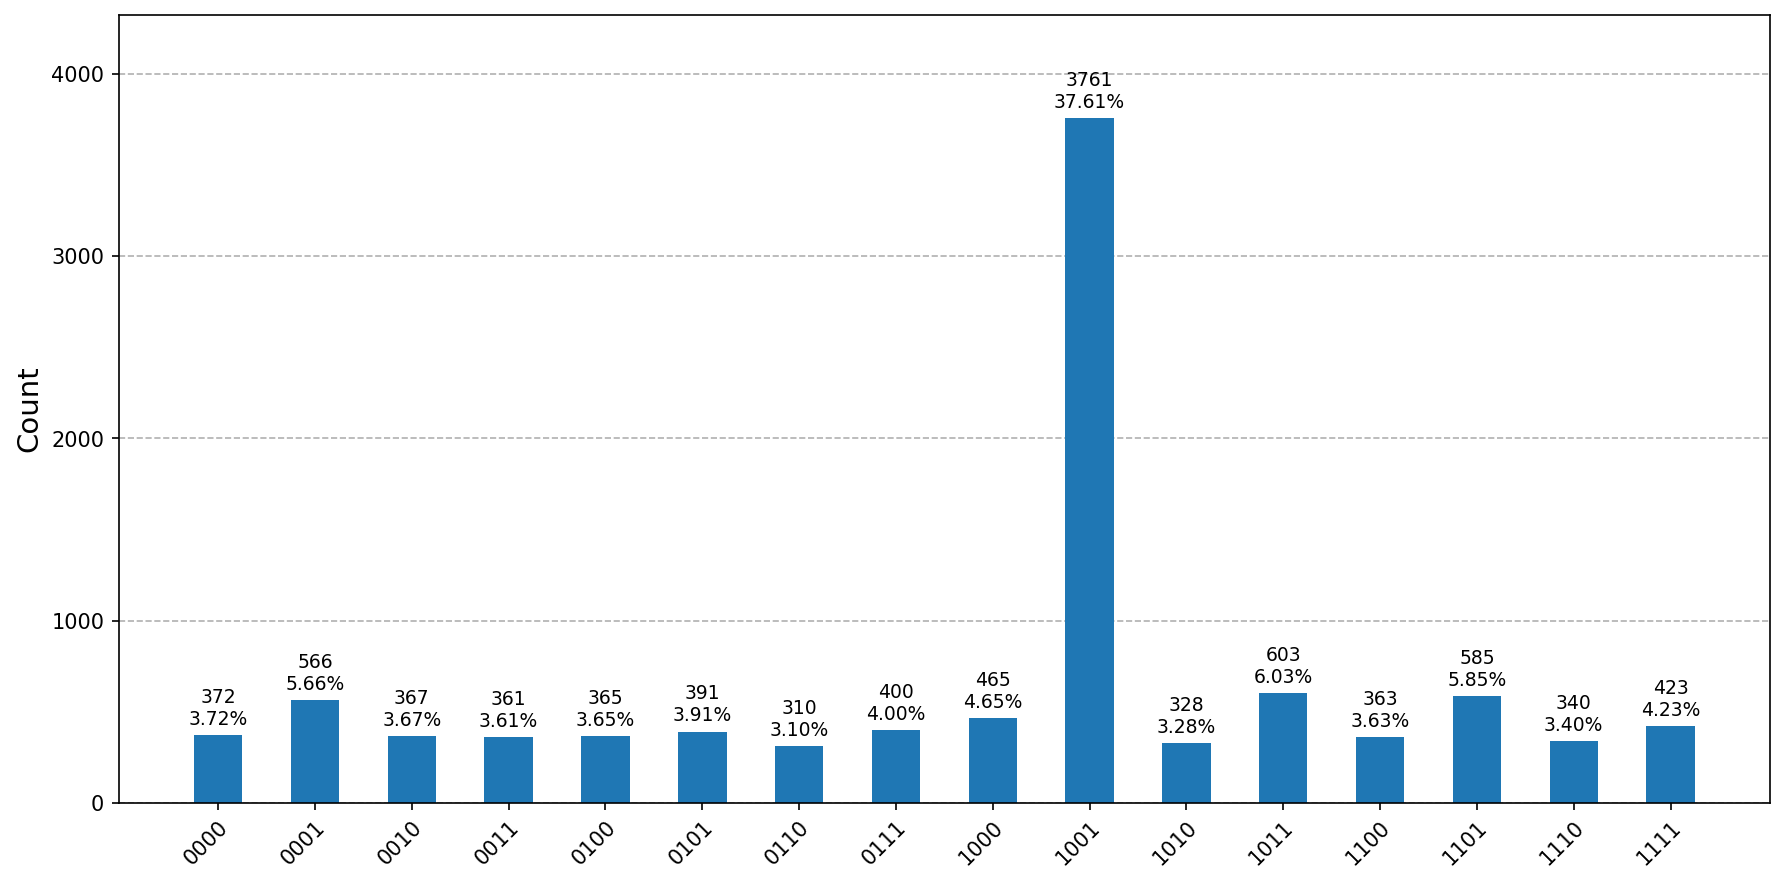
\includegraphics[width=\columnwidth]{figures/lights_out/fake_marrakesh_10k.png}\\
	{\small (b) \texttt{FakeMarrakesh} (10k shots)}\\[0.8em]
	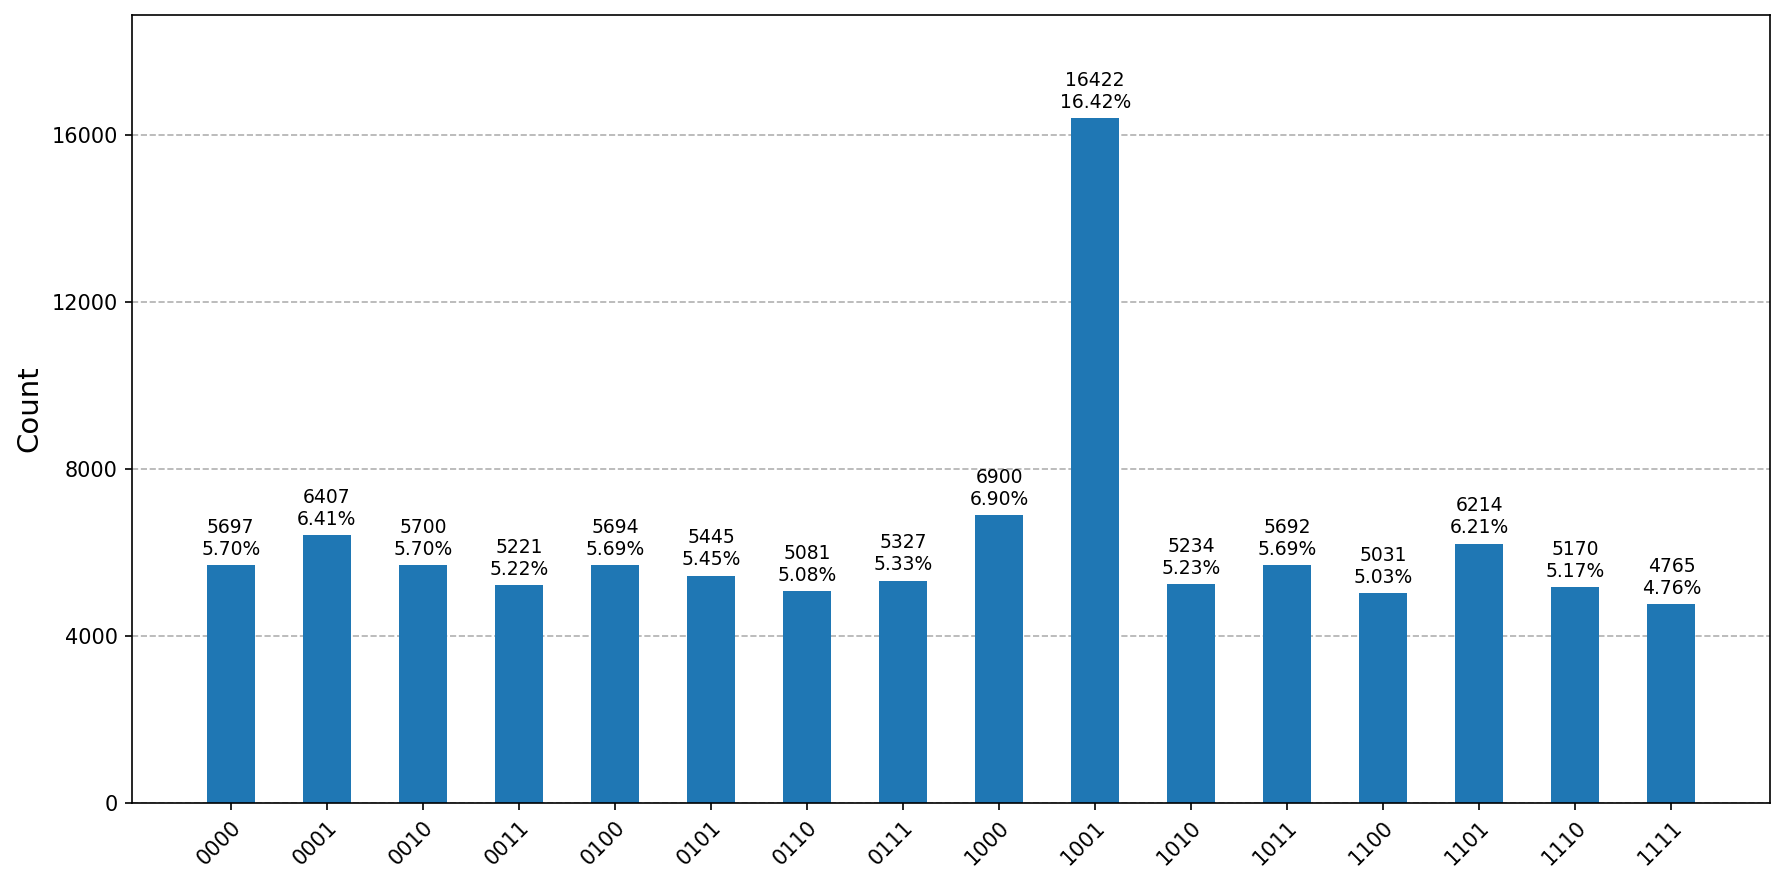
\includegraphics[width=\columnwidth]{figures/lights_out/ibm_marrakesh_100k.png}\\
	{\small (c) IBM hardware (\texttt{ibm\_marrakesh}, 100k shots)}
	\caption{Outcome histograms for the $2\times 2$ Lights Out instance.}
	\label{fig:lights_out_histograms}
\end{figure}


\paragraph{WFC:}

The Wave Function Collapse (WFC) implementation was evaluated on a $3\times 3$ grid, which represents the largest instance that could be handled reliably within the available simulation resources. Even at this size, the problem already exhibits a large number of valid configurations, making it a suitable benchmark to study Grover’s algorithm in a highly degenerate solution space. A quantitative summary of the experiment is therefore given first to establish the computational scale and observed performance.
\\
\\
Table~\ref{tab:wfc_metrics} summarizes the quantum resource requirements and simulation results for the $3\times 3$ instance. The encoding required 18 data qubits to represent tile values and 8 ancilla qubits for reversible constraint checking, resulting in a total of 26 qubits. The logical circuit depth before transpilation was 12, which increased to 2063 after transpilation for the simulator backend. In the noiseless Qiskit simulator, $1020$ out of $1024$ measurement shots corresponded to valid configurations, yielding a success probability of $99.6\%$. In total, 790 unique valid configurations were observed. Example valid tile configurations generated by the quantum algorithm are provided in Appendix~A.

\begin{table}[H]
\centering
\caption{Quantum Wave Function Collapse results for the $3\times 3$ grid.}
\label{tab:wfc_metrics}
\begin{tabular}{l c}
\hline
\textbf{Metric} & \textbf{Value} \\
\hline
Grid size & $3\times 3$ \\
Qubits (data / ancilla / total) & $18 / 8 / 26$ \\
Grover iterations & 9 \\
Circuit depth (pre / post transp.) & $12 / 2063$ \\
Valid outcomes & $1020 / 1024$ (99.6\%) \\
\hline
\end{tabular}
\end{table}

\noindent
To study the behavior of Grover’s algorithm for this problem, the success probability was evaluated as a function of the number of Grover iterations. Figure~\ref{fig:wfc_iterations} shows that, for the iteration range $k=0$ to $k=10$, the success probability follows a smooth rising curve that is consistent with a segment of the expected quadratic sinusoidal behavior. For larger iteration counts, the probability is expected to oscillate according to an overall quadratic sinusoidal envelope, as predicted by Grover theory. This can be seen for the 2x2 grid size shown in Appendix A. The relatively smooth behavior observed here is explained by the large fraction of marked states, which reduces the sharpness of the oscillations compared to problems with a unique solution.

\begin{figure}[htbp]
    \centering
    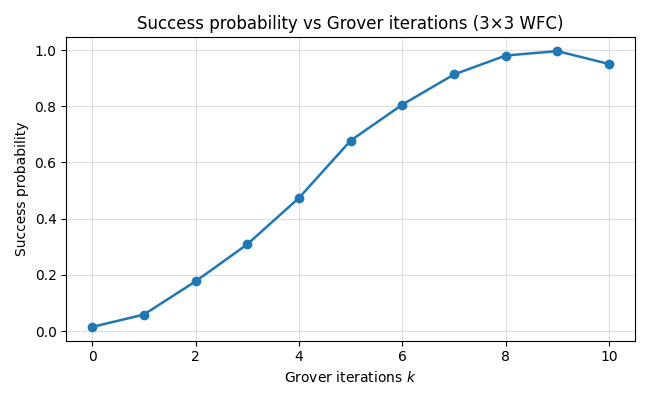
\includegraphics[width=\linewidth]{figures/wfc/Figure_3.png}
    \caption{Measured success probability as a function of the number of Grover iterations for the $3\times 3$ WFC instance.}
    \label{fig:wfc_iterations}
\end{figure}

\vspace{1em}
\noindent
The outcome distributions obtained from simulation and real quantum hardware are compared in Figure~\ref{fig:wfc_histograms}. In the noiseless Qiskit simulator, the top measured outcomes correspond exclusively to valid configurations, each with a probability on the order of $3.5\times10^{-3}$ to $4.0\times10^{-3}$, indicating correct oracle and diffuser behavior. In contrast, execution on IBM quantum hardware shows substantial probability mass distributed over invalid configurations. Out of $1024$ shots on hardware, only $14$ valid configurations were observed, corresponding to a success probability of approximately $1.4\%$. The reason behind this decrease in probability can be seen when looking at the circuit depth. The circuit depth for the simulator case was around 2063, while the IBM hardware increases this to 169580. This is due to the compression of the multi-controlled X and Z gates into elementray gates.

\begin{figure}[h]
	\centering
	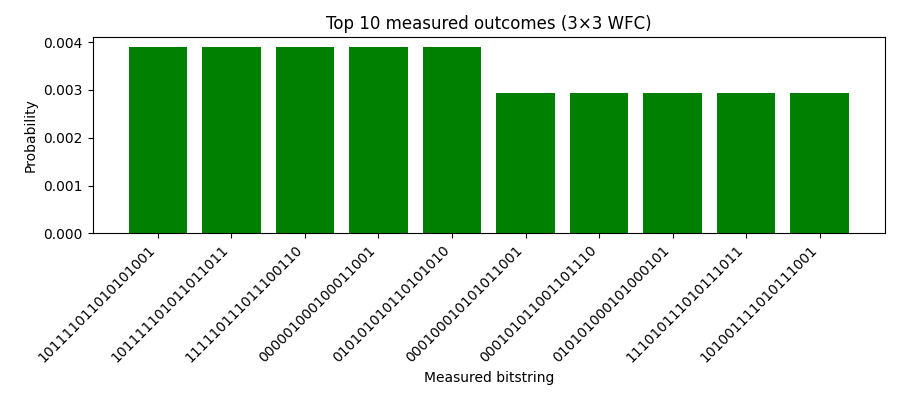
\includegraphics[width=\linewidth]{figures/wfc/Figure_5.png}
	{\small (a) Noiseless Qiskit simulator}\\
	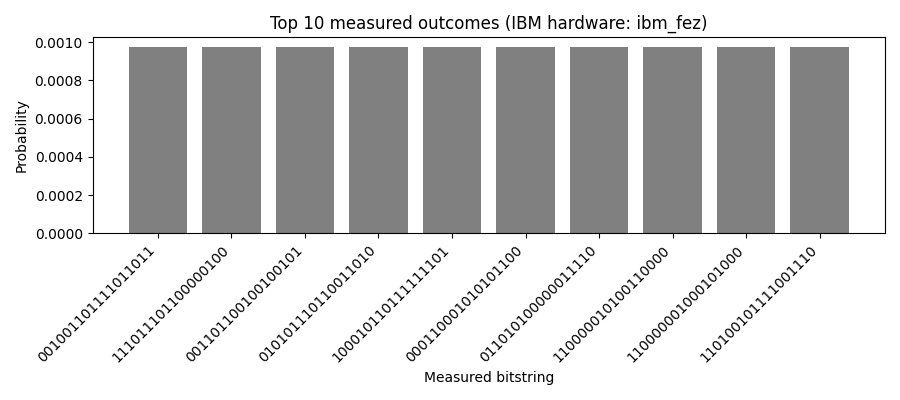
\includegraphics[width=\linewidth]{figures/wfc/Figure_6.png}
	{\small (b) IBM quantum hardware}
	\caption{Measurement histograms for the $3\times 3$ WFC instance. Green bars indicate valid configurations, while gray bars indicate invalid configurations. The simulator amplifies only valid solutions, whereas the hardware distribution is strongly degraded by noise and circuit depth.}
	\label{fig:wfc_histograms}
\end{figure}

\noindent
Finally, the quantum WFC results are compared to a classical WFC implementation. Figure~\ref{fig:wfc_classical} shows an example map generated classically. Classical WFC produces valid $3\times 3$ maps practically instantly. Our implementation has been optimized for our choice of ruleset, and has a runtime complexity of $O(n^4)$ for n by n grids, but for more complex rulesets the complexity may be up to $O(n^5)$. The runtime complexity of the quantum version of WFC is hard to analyze, because the number of valid results is very difficult to calculate for any arbitrary ruleset, which means the exact optimal number of iterations is unknown. In practice, however, the quantum implementation is greatly limited by the depth of the quantum circuit, as too deep circuits cause noise in the measurement result to the point of the result being purely random. We were able to simulate our quantum implementation for grid sizes up to 3 by 3, but all attempts to run the algorithm on actual hardware unfortunately failed. This means that for any grid size, the classical implementation remains superior for now.

\begin{figure}[H]
    \centering
    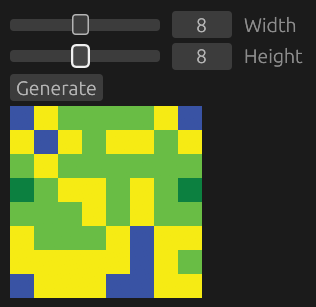
\includegraphics[width=\linewidth]{figures/wfc/Figure_9.png}
    \caption{Example of a tile map generated using our classical Wave Function Collapse solver implementation. Here, Water tiles are in blue, Beach tiles in yellow, Grass tiles in light green and Forest tiles in dark green.}
    \label{fig:wfc_classical}
\end{figure}
